% 左为真实解析曲线；右为两个各10项的完整教学计数。
\begin{tikzpicture}[figure picture,foundation picture]
 \path[use as bounding box] (0,-7) rectangle (163.2,71);
 \node[inner sep=0pt] at (39,33) {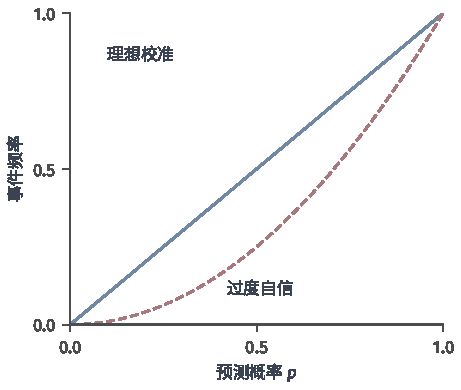
\includegraphics[width=78mm]{figures/02-foundations/03-trustworthiness/tikz/trust-calibration-discrimination/trust-calibration-discrimination.pdf}};
 \node at (124,65) {等大群体：各10项};
 \foreach \k in {0,...,9}{
  \ifnum\k<2 \filldraw[draw=FigureRed,fill=FigureRed,line width=.6pt] ({88+7.8*\k},52) circle(1.6mm);
  \else \draw[draw=FigureBlue,fill=white,line width=.6pt] ({88+7.8*\k},52) circle(1.6mm);\fi
  \ifnum\k<8 \filldraw[draw=FigureRed,fill=FigureRed,line width=.6pt] ({88+7.8*\k},33) circle(1.6mm);
  \else \draw[draw=FigureBlue,fill=white,line width=.6pt] ({88+7.8*\k},33) circle(1.6mm);\fi
 }
 \node at (124,44) {事件频率$2/10=20\%$};
 \node at (124,25) {事件频率$8/10=80\%$};
 \node at (124,14) {常数报告：$0.5,\ 0.5$};
 \node at (124,5) {分组报告：$0.2,\ 0.8$};
 \filldraw[draw=FigureRed,fill=FigureRed] (90,-3) circle(1.3mm);
 \node[foundation note,anchor=west] at (93,-3) {事件发生};
 \draw[draw=FigureBlue,fill=white] (128,-3) circle(1.3mm);
 \node[foundation note,anchor=west] at (131,-3) {未发生};
\end{tikzpicture}
